\section{Actividad No 01 – Comandos} 
¿Que sucede al ejecutar los siguientes comandos? 
\begin{itemize}
\item STARTUP OPEN
	\\Abre los ficheros. Es en este modo cuando podemos decir que la base de datos está
		completamente operativa.
	\\Cuando arrancamos este estado existe la posibilidad de arrancar una misma base de datos
    con distintas instancias, indicando que fichero init.ora queremos que utilice.	
	\item STARTUP MOUNT
	\\Analiza que los ficheros que le indica el parámetro CONTROLFILE en el archivo de
		parámetros, son los que los que se han puesto y que la ruta indicada sea la correcta.
	\\Este estado se usa en caso de que queramos hacer una copia de seguridad de la base de
		datos.
	\\Como en el estado anterior, en modo MOUNT pueden aparecer algunos problemas como los
		siguientes:
		\begin{itemize}
			\item No exista el fichero de control.
			\item Que existan ficheros no sincronizados (lo cual implicaría que se hiciera un 	recover)
			\item No existan los ficheros de datos o de redo log que el CONTROLFILE debe leer. 
			Si el fichero de datos que falta no es crítico, puedo arrancar sin él y después recuperarlo 
			con un backup.
			
		\end{itemize}
	\item STARTUP NOMOUNT
	\\En este estado arrancan los procesos de background y se construye la instancia.
	\\Este estado se emplea para deshabilitar procesos, modificar ficheros de la BD, y recrear el
	fichero de control. En caso de que queramos modificar algún fichero de la base de datos debido a
	que necesitamos por ejemplo si se quieren modificar los archivos de control o los de datos.
	\\Cuando estemos ejecutando este estado se pueden presentar algunos problemas:		
		\begin{itemize}
			\item Problemas de hardware.
			\item Que no exista el fichero de inicialización que le hemos pasado.
			\item Que algunos parámetros del fichero de inicialización estén mal. Si se nos da este
			problema podemos decirle que arranque con el fichero de inicio por defecto llamado	
			init.ora escribiendo el comando STARTUP PFILE = INIT.ora NOMOUNT.			
		\end{itemize}
	\item STARTUP FORCE
	\\Si la base de datos está abierta, FORCE apaga la base de datos con una SHUTDOWN ABORTdeclaración antes de volver a abrirla. 
	\\Si la base de datos está cerrada, entonces FORCE  abre la base de datos.
	\\Puede usar la opción de inicio de STARTUP FORCE si tiene dificultades para iniciar la base de datos de una manera normal. 
	\\Por ejemplo, si un servidor de base de datos perdió energía y la base de datos se detuvo bruscamente, puede dejar la base de datos en un estado en 		el que sea necesario un inicio de STARTUP FORCE. 
	\\Este tipo de inicio normalmente no debería ser requerido, pero puede usarse si un inicio normal no funciona. 
	\\STARTUP FORCE realiza un aborto de apagado y luego reinicia la base de datos.

\vspace*{0.20in}
\vspace*{0.1in}
\begin{large}
Mediante el comando SHUTDOWN podemos apagar una base de datos Oracle. \\
\end{large}
tipos:

\item SHUTDOWN NORMAL
	\\Realiza un cierre consistente de la base de datos de destino con prioridad normal (opción predeterminada), lo que significa:
		
		\begin{itemize}
			\item No se permiten nuevas conexiones después de la emisión de la declaración.
			\item Antes de apagarse, la base de datos espera a que los usuarios conectados actualmente se desconecten
			\item El próximo inicio de la base de datos no requerirá la recuperación de la instancia.
			
		\end{itemize}
\item SHUTDOWN TRANSACTIONAL
	\\Realiza un cierre constante de la base de datos de destino al tiempo que minimiza la interrupción para los clientes, con las siguientes consecuencias:
		
		\begin{itemize}
			\item Los clientes que actualmente realizan transacciones pueden completar, es decir, confirmar o finalizar antes del cierre.
			\item Ningún cliente puede iniciar una nueva transacción en esta instancia; Se desconecta cualquier cliente que intente iniciar una nueva transacción
			\item Después de que todas las transacciones se hayan confirmado o finalizado, cualquier cliente que aún esté conectado se desconectará.		
		\end{itemize}
\item STARTUP RESTRICTT 
	\\Solo permite a los usuarios de Oracle Database con el privilegio del sistema RESTRICTED SESSION conectarse a la base de datos. M\'as tarde, puede usar el comando ALTER SYSTEM 
	\\para deshabilitar la caracter\'istica de sesi\'on restringida.
	\\
\item STARTUP RECOVER 
	\\Especifica que se debe realizar la recuperación de medios, si es necesario, antes de iniciar la instancia. STARTUP RECOVER tiene el mismo efecto que emitir el comando RECOVER
	 \\DATABASE e iniciar una instancia. Solo es posible la recuperaci\'on completa con la opci\'on RECUPERAR.
	\\La recuperaci\'on contin\'ua, si es necesario, como si AUTORECOVERY estuviera configurado en ON, independientemente de si AUTORECOVERY est\'a habilitado o no. Si no se encuentra 
	\\un archivo de registro de rehacer en la ubicaci\'on esperada, la recuperaci\'on contin\'ua como si AUTORECOVERY estuviera deshabilitado, solicit\'andole la ubicaci\'on sugerida y el nombre 
	\\de los archivos de registro posteriores que deben aplicarse.


          \item SHUTDOWN INMEDIATE
	       \\Quizás la mejor manera de cerrar inicialmente la base de datos es el comando de SHUTDOWN INMEDIATE . Este comando evitará los nuevos inicios de sesión, luego revertirá las transacciones no confirmadas y luego desactivará la base de datos. En el proceso de derribar la base de datos, Oracle también descargará todos los cambios en la memoria a los archivos de datos de la base de datos, al igual que lo hace un cierre regular.
                  \\ Esto hace que el inicio de la base de datos sea más rápido.
 Este es un ejemplo de cierre de una base de datos con el comando de cierre inmediato:
                      \begin{figure}[htb]
                      \begin{center}
                      
\includegraphics[width=8cm]{./Imagenes/shutdown_inmediate}
                      \end{center}
                      \end{figure}
        \\item SHUTDOWN ABORTT
                   \\El comando shutdown abort es prácticamente una forma garantizada de cerrar la base de datos. Es un "bloqueo duro" de la base de datos, y esto puede resultar en un tiempo más largo para iniciar la copia de seguridad de la base de datos. Aún así, no puede dañar la base de datos con el comando shutdown abort, y durante sus años de DBA encontrará más de unas pocas ocasiones para usar el comando shutdown abort .
                     \\Un shutdown abort  puede ser su primer método de elección, ya que puede haber ocasiones en las que deba forzar el cierre de la base de datos. Aquí hay un ejemplo usando el comando shutdown abort:
                      \begin{figure}[htb]
                      \begin{center}
                      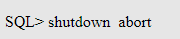
\includegraphics[width=8cm]{./Imagenes/shutdown_abort}
                      \end{center}
                      \end{figure}
\end{itemize} 